%% ------------------------------------------------------------------------- %%
\chapter{Métodos Ágeis Abertos para o OMM}
\label{cap:omm}

O objetivo do projeto QualiPSo\footnote{\url{http://www.qualipso.org}
  - Último acesso em 27/08/2010} é de aumentar a confiabilidade da
indústria e a qualidade dos sistemas livres existentes e futuros. Para
atingir esse objetivo, o projeto conta com 10 grandes áreas de
trabalho. Uma dessas áreas é relacionado à confiabilidade do processo
usado no desenvolvimento de projetos livres.

Desde o início, o projeto abraçou o fato de que não poderia jamais
forçar uma forma de trabalho a comunidades livres. Por isso, a
abordagem usada para aumentar essa confiabilidade foi estabelecer uma
forma de avaliar a qualidade do processo usado por um determinado
projeto livre. Sendo assim, o projeto procurou elaborar um selo que
pudesse ser dado às comunidades que estivesse de acordo com um modelo
de processo confiável.

Porém, o contexto de projetos livre difere (como foi apresentado
anteriormente) do contexto para ambientes empresariais comuns. Por
isso, modelos de avaliação de processos estabelecidos na indústria não
são adequados para ambientes livres. Por isso, decidiu-se elaborar o
modelo de maturidade para software livre do Qualipso (\textit{QualiPSo
  Opensource Maturity Model} - OMM).

A seção \ref{sec:o-que-eh-omm} apresenta mais detalhes da origem do
OMM e de sua constituição. Em seguida, a seção \ref{sec:xp-em-omm}
apresenta como programação extrema pode ser mapeada para o OMM e quais
são os pontos não tratados. Por fim, a seção
\ref{sec:openagile-em-omm} apresenta uma sugestão de práticas
complementares para permitir a aprovação no OMM.

\section{Origem e descrição do OMM}
\label{sec:o-que-eh-omm}

O OMM se baseia na ideia de que a indústria confia em certificados de
qualidade. Padrões como o selo
ISO9001\footnote{\url{http://www.iso.org/} - Último acesso em
  27/08/2010} ou como o Modelo de Maturidade de Capabilidade
(\textit{Capability Maturity Model} - CMM) do Instituto de Engenharia
de Software ( \textit{Software Engineering Institute} - SEI)
\footnote{\url{http://www.sei.cmu.edu/cmmi} - Último acesso em
  27/08/2010} são constituídos de documentos que descrevem uma lista
de exigências que precisam ser cumpridas pelo processo das empresas
que esperaraem obter o selo.

Como projetos livres raramente beneficiam de uma infraestrutura física
ou organizacional, é muito difícil avaliar esses processos de acordo
com esses padrões da indústria. Por isso, o QualiPSo propôs trabalhar
num modelo baseado no CMM mas que pudesse ser usado não apenas para
empresas que incluem software livre em suas soluções mas também pelas
comunidades livres ao redor do mundo. Desse fato, decorre uma nota
importante sobre o OMM. O modelo todo foi pensado para que fosse
simples e fácil de usar pelos vários níveis organizacionais existentes
no ambiente de softwre livre.

A primeira fase de elaboração do OMM foi realizar um levantamento dos
chamados elementos de confiabilidade (\textit{Trusthworthy elements})
no contexto de software livre. Os elementos identificados formaram a
base do OMM para garantir que o processo avaliado não apresentasse
apenas qualidade e confiabilidade do ponto de vista comercial mas
também no contexto de comunidades livres.

Levantados esses elementos de confiabilidade, a equipe do OMM realizou
um mapeamento das áreas de qualidades avaliadas no CMM para
identificar quais elementos eram abordados e quais não eram. Os
principais elementos de confiabilidade que o CMM não aborda estão
relacionados aos problemas legais do uso de software e à reputação de
determinado projeto além do tamanho de sua comunidade.

No aspecto legal, as questões do licenciamento do código, da violação
de patentes e preservação de marcas são pontos importantíssimos para
permitir o uso de qualquer projeto livre numa organização
comercial. Na questão das contribuições, é importante tomar cuidado
com a questão dos direitos autorais para evitar problemas legais
relacionados ao licenciamento do código.  Esses dois aspectos não são
tratados ou sequer abordados no CMM porque a existência de uma
organização responsável por qualquer desenvolvimento e de regras
contratuais estabelecidas evita esses problemas.

Por outro lado, o CMM aborda alguns aspectos que são importantes para
a confiabilidade de um projeto no contexto comercial. Muitos desses
aspectos estão ligados a exigências na quantidade e detalhamento de
documentos usados para inspeção e melhoria dentro da organização que
implementa o processo. A equipe do OMM selecionou todas as práticas
sugeridas pelo CMM no que diz respeito aos aspectos técnicos e apenas
algumas no aspecto gerencial que fizessem sentido no contexto livre.

Graças a esse trabalho, o OMM foi formado com um misto de elementos de
confiabilidade vindos da comunidade de software livre com práticas
estabelecidas vindas do CMM. O modelo ainda optou por adotar uma
estrutura piramidal semelhante à do CMM na qual existem três níveis de
adequação sendo que o mais básico é base para os mais avançados que
sempre exigem todas as práticas do nível inferior e mais algumas.

A figura \ref{fig:piramide-omm} apresenta a divisão de níveis com a
lista de práticas (com nomes abreviados) que integra cada um dos
níveis do OMM. Além disso, o OMM propõe exigências diferentes de
acordo com o tipo de entidade que deseja ser avaliada para um
determinado nível. Isto é, algumas práticas são apenas recomendadas e
não obrigatórias para comunidades livres não representadas por uma
empresa. Dessa forma, quando o projeto não tem uma organização por
trás, os membros da comunidade só precisam realizar o que está no
alcance de uma comunidade para atingir um determinado nível.

% TODO Traduzir figura
\begin{figure}
  \centering
  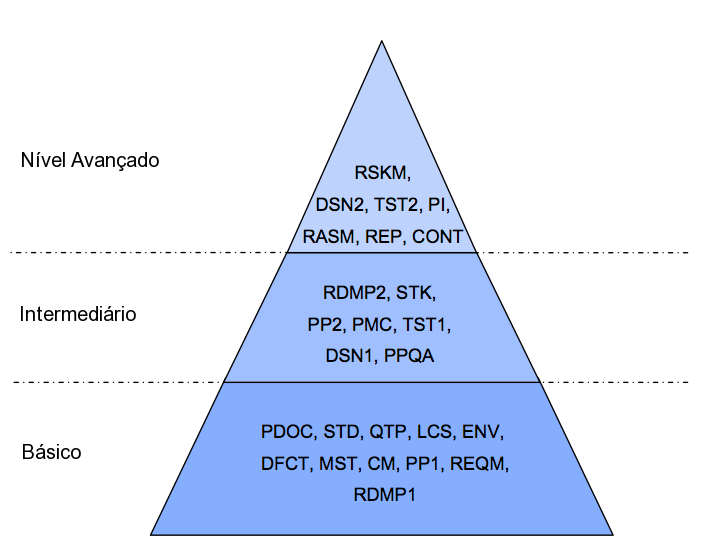
\includegraphics[scale=0.4]{omm-levels}
  \caption{Pirâmide de práticas exigidas para cada um dos níveis do
    OMM}
  \label{fig:piramide-omm}
\end{figure}

As tabelas \ref{tab:omm-basic}, \ref{tab:omm-intermediate} e
\ref{tab:omm-advanced} mostram os elementos de confiabilidade que
precisam ser endereçados para se atingir os níveis básico,
intermediário e avançados do OMM.

\begin{table}
  \begin{tabular}{|p{2cm}|p{14cm}|}
    \hline
    PDOC & Documentação do Produto (\textit{Product Documentation}) \\
    \hline
    STD & Uso de Padrões Estabelecidos e Adotados (\textit{Use of
      Established and Widespread Standards}) \\
    \hline
    QTP & Qualidade do Plano de Testes (\textit{Quality of Test Plan})
    \\
    \hline
    LCS & Licenças (\textit{Licenses}) \\
    \hline
    ENV & Ambiente Técnico (\textit{Technical Environment} -
    Ferramentas, Sistema Operacional, Linguagem de Programação,
    Ambiente de Desenvolvimento.) \\
    \hline
    DFCT & Número de Commits e Relatórios de \textit{Bugs}
    (\textit{Number of Commits and Bug Reports}) \\
    \hline
    MST & Facilidade de Manutenção e Estabilidade
    (\textit{Maintainability and Stability}) \\
    \hline
    CM & Gestão de configuração
    (\textit{Configuration Management}) \\
    \hline
    PP1 & Planejamento de Projeto Parte 1
    (\textit{Project Planning Part 1}) \\
    \hline
    REQM & Gestão de Requisitos
    (\textit{Requirements Management}) \\
    \hline
    RDMP1 & Disponibilidade de um plano
    (\textit{Availability of a Roadmap}) \\
    \hline
  \end{tabular}
  \caption{Elementos essenciais no nível básico do OMM}
  \label{tab:omm-basic}
\end{table}

\begin{table}
  \begin{tabular}{|p{2cm}|p{14cm}|}
    \hline
    RDMP2 & Desenvolvimento de um plano
    (\textit{Implementation of a Roadmap}) \\
    \hline
    STK & Relações entre interessados
    (\textit{Relationship between Stakeholders} - Usuários,
    Desenvolvedores etc) \\
    \hline
    PP2 & Planejamento de Projeto Parte 2
    (\textit{Project Planning Part 2}) \\
    \hline
    PMC & Monitoramento e Controle do Projeto
    (\textit{Project Monitoring and Control}) \\
    \hline
    TST1 & Testes Parte 1
    (\textit{Test Part 1}) \\
    \hline
    DSN1 & Projeto Parte 1
    (\textit{Design Part 1}) \\
    \hline
    PPQA & Garantia de Qualidade no Processo e no Projeto
    (\textit{Process and Project Quality Assurance}) \\
    \hline
  \end{tabular}
  \caption{Elementos essenciais no nível intermediário do OMM}
  \label{tab:omm-intermediate}
\end{table}

\begin{table}
  \begin{tabular}{|p{2cm}|p{14cm}|}
    \hline
    PI & Integração do Produto
    (\textit{Product Integration}) \\
    \hline
    RSKM & Gestão de Risco
    (\textit{Risk Management}) \\
    \hline
    TST2 & Testes Parte 2
    (\textit{Tests Part 2}) \\
    \hline
    DSN2 & Projeto Parte 2
    (\textit{Design Part 2}) \\
    \hline
    RASM & Resultados das Avaliações de Terceiros
    (\textit{Results of $3^{rd}$ Party Assessments}) \\
    \hline
    REP & Reputação
    (\textit{Reputation}) \\
    \hline
    CONT & Contribuições
    (\textit{Contributions}) \\
    \hline
  \end{tabular}
  \caption{Elementos essenciais no nível avançado do OMM}
  \label{tab:omm-advanced}
\end{table}

O texto do OMM apresenta uma abordagem Objetivo-Pergunta-Métrica (GQM
- \textit{Goal Question Metric}) no qual cada elemento possui um
conjunto de objetivos que precisam ser alcançados (ou não, dependendo
do tipo de organização sendo avaliada). As perguntas são mapeadas para
práticas recomendadas com detalhes de itens que deveriam ser
encontrados para validar que a prática é seguida.

O resto do documento de descrição do OMM apresenta recomendações para
os diferentes tipos de entidades que poderiam se interessar em obter
uma certificação OMM. Também existe uma descrição extensa de como deve
ser realizada a avaliação de uma entidade com um questionário e
informações sobre como cada prática pode ser avaliada.

A próxima seção apresenta como a Programação Extrema descrita por Kent
Beck pode ser mapeada para os elementos de confiabilidade necessários
em cada nível do OMM.

\section{Um mapeamento de Programação Extrema para o OMM}
\label{sec:xp-em-omm}

A tabela \ref{tab:xp-to-omm} apresenta um mapeamento das práticas de
Programação Extrema para os elementos descritos no OMM com as práticas
recomendadas em cada item.

\begin{longtable}{|p{2cm}|p{7cm}|p{7cm}|}
  \caption{Mapeamento de práticas de documenção necessárias no OMM com
    programação extrema} \\
  \multicolumn{3}{|c|}{\cellcolor[gray]{0.6}  Documentação do Produto}\\
  \endhead
  & & \\
  \hline \cellcolor[gray]{0.6} Objetivo PDOC 1 & \cellcolor[gray]{0.6}
  Prover documentação de alta qualidade & Prática de Programação Extrema \\
  \hline \cellcolor[gray]{0.9} Prática PDOC 1.1 &
  \cellcolor[gray]{0.9}
  Criar documentação para desenvolvedores & \\
  \hline \multirow{5}{*}{Procurar} & Disponibilidade de especificações
  de requisitos & Desenvolvimento Dirigido por Comportamento (BDD -
  \textit{Behavior
    Driven Development}) \\
  \cline{2-3} & Disponibilidade de um projeto de alto nível / de uma
  arquitetura do produto & Desenvolvimento Dirigido por Testes (TDD -
  \textit{Test
    Driven Development}) \\
  \cline{2-3} & Disponibilidade de um projeto detalhado &
  Desenvolvimento Dirigido por Testes (TDD - \textit{Test
    Driven Development}) \\
  \cline{2-3} & Disponibilidade de documentação técnica &
  Desenvolvimento Dirigido por Comportamento (BDD - \textit{Behavior
    Driven Development}) \\
  \cline{2-3} & Disponibilidade de guias para o fluxo de trabalho &
  (TDD -
  \textit{Test Driven Development}) \\
  \hline \cellcolor[gray]{0.9} Prática PDOC 1.2 &
  \cellcolor[gray]{0.9}
  Criar documentação para usuários & \\
  \hline \multirow{3}{*}{Procurar} & Disponibilidade de um guia para
  usuário &
  \textbf{Nenhuma} \\
  \cline{2-3} & Disponibilidade de documentos de perguntas frequentes
  &
  \textbf{Nenhuma} \\
  \cline{2-3} & Disponibilidade de material de treinamento sobre como
  usar o produto (material de alcance multimídia) &
  \textbf{Nenhuma} \\
  \hline \cellcolor[gray]{0.9} Prática PDOC 1.3 &
  \cellcolor[gray]{0.9}
  Criar documentação genérica & \\
  \hline \multirow{3}{*}{Procurar} & Disponibilidade de documentos de
  planejamento &
  Planejamento da Iteração (\textit{Iteration Planning}) \\
  \cline{2-3} & Disponibilidade de uma lista de todos os documentos
  disponíveis &
  \textbf{Nenhuma} \\
  \cline{2-3} & Disponibilidade de livros descrevendo o projeto
  (número, linguagem...) &
  \textbf{Nenhuma} \\
  \hline
  & & \\
  \hline \cellcolor[gray]{0.6} Objetivo PDOC 2 & \cellcolor[gray]{0.6}
  Criar documentação pro produto & Prática de Programação Extrema \\
  \hline \cellcolor[gray]{0.9} Prática PDOC 2.1 &
  \cellcolor[gray]{0.9}
  Prover um sistema de documentação & \\
  \hline \multirow{2}{*}{Procurar} & Disponibilidade de uma
  funcionalidade de indexação de funcionalidades (buscando
  palavras-chave por exemplo) &
  \textbf{Nenhuma} \\
  \cline{2-3} & Disponibilidade de um sistema de gestão de
  documentação integrado &
  \textbf{Nenhuma} \\
  \hline \cellcolor[gray]{0.9} Prática PDOC 2.2 &
  \cellcolor[gray]{0.9} Manter toda documentação acima baseado no
  \textit{feedback}
  coletado dos usuários com relação à documentação. & \\
  \hline \multirow{2}{*}{Procurar} & Disponibilidade de um sistema de
  avaliação da documentação &
  \textbf{Nenhuma} \\
  \cline{2-3} & Disponibilidade de um conjunto de páginas wiki, fóruns
  ou listas de email dedicados à documentação do projeto&
  \textbf{Nenhuma} \\
  \hline
  & & \\
  \hline \cellcolor[gray]{0.6} Objetivo PDOC 3 & \cellcolor[gray]{0.6}
  Melhorar a documentação do produto & Prática de Programação Extrema \\
  \hline \cellcolor[gray]{0.9} Prática PDOC 3.1 &
  \cellcolor[gray]{0.9}
  Planejamento de documentação & \\
  \hline \multirow{4}{*}{Procurar} & Disponibilidade de um
  planejamento detalhado de criação de documentação &
  \textbf{Nenhuma} \\
  \cline{2-3} & Garantir que a documentação é apropriada para a versão
  do produto &
  \textbf{Nenhuma} \\
  \cline{2-3} & Verificar a qualidade da apresentação da documentação
  &
  \textbf{Nenhuma} \\
  \cline{2-3} & Verificar a qualidade da apresentação do
  \textit{feedback} dos usuários &
  \textbf{Nenhuma} \\
  \hline \cellcolor[gray]{0.9} Prática PDOC 3.2 &
  \cellcolor[gray]{0.9}
  Melhorar o suporte para várias linguagens naturais & \\
  \hline \multirow{1}{*}{Procurar} & Disponibilidade de documentação
  em diferentes linguagens &
  \textbf{Nenhuma} \\
  \hline \cellcolor[gray]{0.9} Prática PDOC 3.3 &
  \cellcolor[gray]{0.9}
  Melhorar a disponibilidade da documentação & \\
  \hline \cellcolor[gray]{0.9} Prática PDOC 3.4 &
  \cellcolor[gray]{0.9} Melhorar os documentos baseado no
  \textit{feedback} e na avaliação
  &   \label{tab:xp-to-omm} \\
  \hline
\end{longtable}

\begin{longtable}{|p{2cm}|p{7cm}|p{7cm}|}
  \caption{Mapeamento de práticas de adoção de padrões necessárias no
    OMM com
    programação extrema} \\
  \multicolumn{3}{|c|}{\cellcolor[gray]{0.6} Uso de Padrões
    Estabelecidos e Difundidos}\\
  \endhead
  & & \\
  \hline \cellcolor[gray]{0.6} Objetivo STD 1 & \cellcolor[gray]{0.6}
  Aderir a Padrões Abertos & Prática de Programação Extrema \\
  \hline \cellcolor[gray]{0.9} Prática STD 1.1 & \cellcolor[gray]{0.9}
  Aderir a padrões do produto (Padrões Abertos) & \\
  \hline \multirow{9}{*}{Procurar} & Aderir a padrões abertos na área
  de: - Redes (TCP/IP, SSL, SMTP, MIME, IMAP, LDAP, WWW-HTTP...) &\textbf{Nenhuma} \\
  \cline{2-3} & - Conteúdos \textit{Web} (HTML...) &\textbf{Nenhuma} \\
  \cline{2-3} & - Email (SMTP, Email, WWW-MIME...) &\textbf{Nenhuma}
  \\
  \cline{2-3} & - Troca de documentos (XML...) &\textbf{Nenhuma} \\
  \cline{2-3} & - Gráficos (PNG...) &\textbf{Nenhuma} \\
  \cline{2-3} & - Sistemas de Janelas (X Window...) &\textbf{Nenhuma}
  \\
  \cline{2-3} & - Audio (Ogg, Vorbis...) &\textbf{Nenhuma} \\
  \cline{2-3} & - Documentos de Escritório (OpenDocument...)
  &\textbf{Nenhuma} \\
  \cline{2-3} & - Serviços \textit{Web} (UDDI, SOAP...) &\textbf{Nenhuma} \\
  \hline \cellcolor[gray]{0.9} Prática STD 1.2 & \cellcolor[gray]{0.9}
  Aderir a padrões de produtos de boa qualidade (Padrões Abertos) & \\
  \hline \multirow{3}{*}{Procurar} & Aderir padrões bem estabelecidos
  &
  \textbf{Nenhuma} \\
  \cline{2-3} & Aderir a parões altamente inter-operáveis &
  \textbf{Nenhuma} \\
  \cline{2-3} & Aderir a parões amplamente difundidos &
  \textbf{Nenhuma} \\
  \hline \cellcolor[gray]{0.9} Prática STD 1.3 & \cellcolor[gray]{0.9}
  Garantir a satisfação do usuário com os padrões usados no projeto & \\
  \hline \multirow{8}{*}{Procurar} & Baseado no nível de satisfação
  dos usuários com relação aos padrões usados &
  \textbf{Nenhuma} \\
  \cline{2-3} & Baseado no nível de satisfação dos desenvolvedores com
  relação aos padrões usados& \textbf{Nenhuma} \\
  \cline{2-3} & Realizar uma verificação de inter-operabilidade dos
  novos componentes e padrões usados no projeto & \textbf{Nenhuma} \\
  \cline{2-3} & Verificar a satisfação dos usuários com a
  inter-operabilidade dos formatos de dados & \textbf{Nenhuma} \\
  \cline{2-3} & Verificar a satisfação dos usuários com a
  inter-operabilidade dos fluxos de trabalho & \textbf{Nenhuma} \\
  \cline{2-3} & Verificar a satisfação dos usuários com a
  inter-operabilidade das interfaces de programação & \textbf{Nenhuma}
  \\
  \cline{2-3} & Verificar a satisfação dos usuários com a
  inter-operabilidade das interfaces com o usuário & \textbf{Nenhuma}
  \\
  \cline{2-3} & Verificar a satisfação dos usuários com a
  inter-operabilidade das interfaces dos protocolos de comunicação &
  \textbf{Nenhuma} \\
  \hline \cellcolor[gray]{0.9} Prática STD 1.4 & \cellcolor[gray]{0.9}
  Aderir a padrões certificados por entidades certificadoras que
  apoiem Software Livre & \\
  \hline \multirow{1}{*}{Procurar} & O projeto adere a padrões
  propostos pelas seguintes entidades de certificação: IETF, IEEE,
  OASIS, W3C, Free Standards Group, outras entidades que apoiam
  Software Livre &
  \textbf{Nenhuma} \\
  \hline \cellcolor[gray]{0.9} Prática STD 1.5 & \cellcolor[gray]{0.9}
  Documente padrões do produto & \\
  \hline \multirow{1}{*}{Procurar} & & \\
  \hline
  & & \\
  \hline \cellcolor[gray]{0.6} Objetivo STD 2 & \cellcolor[gray]{0.6}
  Adote processos de desenvolvimento padrões & Prática de Programação Extrema \\
  \hline \cellcolor[gray]{0.9} Prática STD 2.1 & \cellcolor[gray]{0.9}
  Aderir a padrões abertos para o processo & \\
  \hline \multirow{2}{*}{Procurar} & Garantir a conformidade de
  algumas atividades ao processo &
  \textbf{Nenhuma} \\
  \cline{2-3} & Garantir o uso de mecanismos para controlar o processo
  (i.e. baseados no ISO9000, CMMI, SPICE etc)&
  \textbf{Nenhuma} \\
  \hline \cellcolor[gray]{0.9} Prática STD 2.2 & \cellcolor[gray]{0.9}
  Avaliar o processo baseado numa abordagem de
  avaliação amplamente difundida & \\
  \hline \multirow{2}{*}{Procurar} & O planejamento do projeto inclui
  avaliações agendadas para garantir a aderência ao processo &
  \textbf{Nenhuma} \\
  \cline{2-3} & Resultados da avaliação são apresentados aos usuários
  &
  \textbf{Nenhuma} \\
  \hline
  & & \\
  \hline \cellcolor[gray]{0.6} Objetivo STD 3 & \cellcolor[gray]{0.6}
  Garanta independência estratégica do projeto & Prática de Programação Extrema \\
  \hline \cellcolor[gray]{0.9} Prática STD 3.1 & \cellcolor[gray]{0.9}
  Independência de tecnologias específicas & \\
  \hline \multirow{5}{*}{Procurar} & Independência de padrões
  proprietários &
  \textbf{Nenhuma} \\
  \cline{2-3} & Independência de ferramentas de desenvolvimento
  proprietárias &
  \textbf{Nenhuma} \\
  \cline{2-3} & Independência de módulos e componentes de software
  proprietários &
  \textbf{Nenhuma} \\
  \cline{2-3} & Independência de formatos de dados proprietários &
  \textbf{Nenhuma} \\
  \cline{2-3} & Independência do projeto de possíveis futuros
  travamentos &
  \textbf{Nenhuma} \\
  \hline
\end{longtable}

\begin{longtable}{|p{2cm}|p{7cm}|p{7cm}|}
  \caption{Mapeamento de práticas de qualidade de testes necessárias
    no OMM com programação extrema} \\
  \multicolumn{3}{|c|}{\cellcolor[gray]{0.6} Qualidade do Processo de Testes}\\
  \endhead
  & & \\
  \hline \cellcolor[gray]{0.6} Objetivo QTP 1 & \cellcolor[gray]{0.6}
  Prover um plano de alta qualidade de testes & Prática de Programação Extrema \\
  \hline \cellcolor[gray]{0.9} Prática QTP 1.1 & \cellcolor[gray]{0.9}
  Garantir que o plano de testes cubra testes funcionais & \\
  \hline \cellcolor[gray]{0.9} Prática QTP 1.2 & \cellcolor[gray]{0.9}
  Garantir que o plano de testes cubra testes não-funcionais (como
  exigido pelo projeto; veja abaixo) & \\
  \hline \multirow{9}{*}{Procurar} & Escalabilidade &\textbf{Nenhuma} \\
  \cline{2-3} & Manutenibilidade &\textbf{Nenhuma} \\
  \cline{2-3} & Usabilidade &\textbf{Nenhuma} \\
  \cline{2-3} & Desempenho &\textbf{Nenhuma} \\
  \cline{2-3} & Segurança &\textbf{Nenhuma} \\
  \cline{2-3} & Estabilidade &\textbf{Nenhuma} \\
  \cline{2-3} & Testabilidade &\textbf{Nenhuma} \\
  \cline{2-3} & Internacionalização/Localização &\textbf{Nenhuma} \\
  \cline{2-3} & Outros testes não-funcionais exigidos pelo projeto
  específico &\textbf{Nenhuma} \\
  \hline \cellcolor[gray]{0.9} Prática QTP 1.3 & \cellcolor[gray]{0.9}
  Garantir que o plano de testes cubra diferentes abordagens de teste,
  considere: & \\
  \hline \multirow{4}{*}{Procurar} & testes de unidade
  & \textbf{Nenhuma} \\
  \cline{2-3} & testes de integração & \textbf{Nenhuma} \\
  \cline{2-3} & testes de sistema & \textbf{Nenhuma} \\
  \cline{2-3} & testes de integração de sistema & \textbf{Nenhuma} \\
  \hline \cellcolor[gray]{0.9} Prática QTP 1.4 & \cellcolor[gray]{0.9}
  Definir casos de teste e critérios de teste, considere: & \\
  \hline \multirow{4}{*}{Procurar} & requisitos de usuário &
  \textbf{Nenhuma} \\
  \cline{2-3} & requisitos de arquitetura & \textbf{Nenhuma} \\
  \cline{2-3} & requisitos técnicos & \textbf{Nenhuma} \\
  \cline{2-3} & requisitos do processo de testes & \textbf{Nenhuma} \\
  \hline
  & & \\
  \hline \cellcolor[gray]{0.6} Objetivo QTP 2 & \cellcolor[gray]{0.6}
  Implementar e gerir o processo de testes & Prática de Programação Extrema \\
  \hline \cellcolor[gray]{0.9} Prática QTP 2.1 & \cellcolor[gray]{0.9}
  Realizar testes frequentemente & \\
  \hline \multirow{2}{*}{Procurar} & Realizar testes diferentes
  frequentemente &
  \textbf{Nenhuma} \\
  \cline{2-3} & Alinhar o processo de testes com o planejamento do
  projeto & \textbf{Nenhuma} \\
  \hline \cellcolor[gray]{0.9} Prática QTP 2.2 & \cellcolor[gray]{0.9}
  Garantir que os recursos de testes (ferramentas, ambiente etc) estão
  claramente definidos & \\
  \hline \multirow{3}{*}{Procurar} & Testes anteriores são claramente
  explicados e os resultados são apresentados &
  \textbf{Nenhuma} \\
  \cline{2-3} & O planejamento de testes futuros é projetado e
  claramente apresentado  &  \textbf{Nenhuma} \\
  \cline{2-3} & \textit{Feedback} é obtido na qualidade do plano de
  testes  &  \textbf{Nenhuma} \\
  \hline \cellcolor[gray]{0.9} Prática QTP 2.3 & \cellcolor[gray]{0.9}
  Melhorar o processo de testes & \\
  \hline \multirow{2}{*}{Procurar} & O projeto provê resultados de
  testes detalhados &
  \textbf{Nenhuma} \\
  \cline{2-3} & \textit{Feedback} dos testes anteriores é obtido e
  está disponível para revisão & \textbf{Nenhuma} \\
  \hline
  & & \\
  \hline \cellcolor[gray]{0.6} Objetivo QTP 3 & \cellcolor[gray]{0.6}
  Melhorar o processo de testes & Prática de Programação Extrema \\
  \hline \cellcolor[gray]{0.9} Prática QTP 3.1 & \cellcolor[gray]{0.9}
  Incluir casos de testes, resultados de testes e considerar
  comentários dos desenvolvedores do projeto livre, considere: & \\
  \hline \multirow{5}{*}{Procurar} & desenvolvedores essenciais &
  \textbf{Nenhuma} \\
  \cline{2-3} & contribuidores ocasionais & \textbf{Nenhuma} \\
  \cline{2-3} & erros identificados & \textbf{Nenhuma} \\
  \cline{2-3} & pedidos funcionais & \textbf{Nenhuma} \\
  \cline{2-3} & ações de desempenho & \textbf{Nenhuma} \\
  \hline \cellcolor[gray]{0.9} Prática QTP 3.2 & \cellcolor[gray]{0.9}
  Incluir casos de testes, resultados de testes e considerar
  comentários dos usuários do produto livre, considere: & \\
  \hline \multirow{3}{*}{Procurar} & erros identificados &
  \textbf{Nenhuma} \\
  \cline{2-3} & pedidos funcionais & \textbf{Nenhuma} \\
  \cline{2-3} & ações de desempenho & \textbf{Nenhuma} \\
  \hline \cellcolor[gray]{0.9} Prática QTP 3.3 & \cellcolor[gray]{0.9}
  Incluir casos de testes, resultados de testes e considerar
  comentários dos integradores do produto livre, considere: & \\
  \hline \multirow{6}{*}{Procurar} & integradores de software livre
  (distribuições de sistema operacional etc) &
  \textbf{Nenhuma} \\
  \cline{2-3} & integradores trabalhando na área de Administração Pública & \textbf{Nenhuma} \\
  \cline{2-3} & integradores baseados na indústria & \textbf{Nenhuma}
  \\
  \cline{2-3} & erros identificados & \textbf{Nenhuma} \\
  \cline{2-3} & pedidos funcionais & \textbf{Nenhuma} \\
  \cline{2-3} & ações de desempenho & \textbf{Nenhuma} \\
  \hline
\end{longtable}


\section{Um proposta ágil compatível com o OMM}
\label{sec:openagile-em-omm}

